\documentclass[a4paper,11pt]{report}
\usepackage[portuguese]{babel}

% * conseguir manusear uma variedade de símbolos usados nos diferentes grupos de línguas
\usepackage[latin1,utf8]{inputenc}

% * colorir textos
\usepackage{graphicx}
% * capa com imagem
\usepackage{titlepic}

% * tamanho das margens
\usepackage{geometry}

% * multiplas colunas
\usepackage{multicol}

% * referencias dentro do ficheiro
\usepackage{hyperref}
\usepackage{xurl}  % * Quebra a url de forma inteligente

% *O Documento tem de ter margens superior e inferior de 1.5 cm e margens
% *   esquerda e direita de 1 cm;
\geometry{a4paper, left= 1 cm, right= 1 cm, top= 1.5 cm, bottom= 1.5 cm }

% * Titulo
\title{
	\Huge{\textbf{Finanças pessoais}} \\
	\vskip 0.25cm \\
	\small{Produção de Documentos Técnicos}
}


% * Data da entrega de trabalho
\date{24 de Novembro de 2024}

% * Nome completo
% * Número de aluno
% * Email
% * Turma que pertence
% * Nome da sua Licenciatura
\author{
	\small{ Arthur Sepulven de Aguiar } \\ 
	\small{ Nº de Aluno 64726 - TP 18 - fc64726@alunos.fc.ul.pt} \\
	\small{Licenciatura em Engenharia Informática}
}

% * Imagem relativa ao tema
\titlepic{
	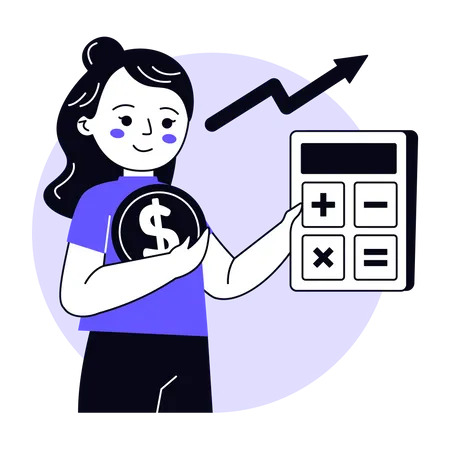
\includegraphics[width=12cm]{./first_page.jpg}
}

% \thispagestyle{empty}

\begin{document}
	% * Todos os índices (conteúdo, tabelas e figuras) são automáticos, 
	% *   feitos pelo LaTeX e estas páginas têm   paginação em numeração romana;
	\pagenumbering{Roman}
	\maketitle

	%  * Índices
	\tableofcontents % * faz o índice

	% * um texto com o máximo de uma página sobre finanças pessoais.
	\chapter{Introdução}
		\begin{multicols}{2}

			\section{Definição \cite{intro:intro}}
				\hspace{1cm} Finanças é a ciência da administração do dinheiro. A gestão financeira pessoal é a maneira na \
				qual se controla e conhece seus gastos e lucros, uma boa gestão consiste no equilíbrio entre receitas e despesas.

			\section{Conseguência das Finanças pessoais \cite{intro:desenvolvimento}}
				\hspace{1cm} A falta de educação financeira pessoal manifesta-se tanto no nível individual quanto no social. \
				Do ponto de vista individual, decisões financeiras impactam diretamente a vida pessoal e familiar,\
				podendo contribuir para uma existência estável ou, ao contrário, gerar instabilidade. \
				Já no contexto social, tais decisões influenciam fatores como a redução da desigualdade, \
				a diminuição da pobreza intergeracional, o estímulo à inovação e ao empreendedorismo. \
				No entanto, quando mal conduzidas, essas decisões podem agravar os mesmos problemas.
			
			\section{Orçamento \cite{intro:orcamento}}
				\hspace{1cm} Criar um orçamento pessoal é um dos primeiros passos para garantir uma gestão financeira eficaz. \
				Para isso, é recomendado que você se eduque financeiramente, avalie suas receitas e despesas, estabeleça \
				metas financeiras, crie um fundo de emergência, divida seu orçamento, ajuste-o regularmente, utilize ferramentas \
				para o controle financeiro e mantenha disciplina. Um orçamento pessoal não precisa ser complexo. Com um pouco de \ 
				educação financeira, organização e disciplina, qualquer indivíduo pode criar um plano eficaz para suas finanças pessoais.

			\section{Conclusão}
				\hspace{1cm} Portanto, o planejamento das despesas e receitas pessoais é imprescindível para qualquer adulto \
				que deseje uma vida estável e sustentável. A gestão das despesas e dos custos vai para além dos efeitos no \
				indivíduo, afetando a sociedade como um todo. Um bom planejamento das finanças tem efeitos que se estendem \
				por várias gerações. Concluo que, de facto, a gestão das finanças pessoais é vantajosa.
		\end{multicols}
	
		\vskip 0.5cm

		\begin{multicols}{2}
			\section{Citação \cite{intro:citacao}} % * Insira também uma citação relativa ao tema.
			\vskip -1cm
			\begin{center}
				\begin{quote}
					\LARGE
					\emph{"The number one problem in today’s generation and economy is the lack of financial literacy."}
				\end{quote}
				\normalsize{O maior problema na geração e economia atual é a falta de literatura financeira.} \\
			\end{center}
			\vskip -1cm
			\begin{center}
				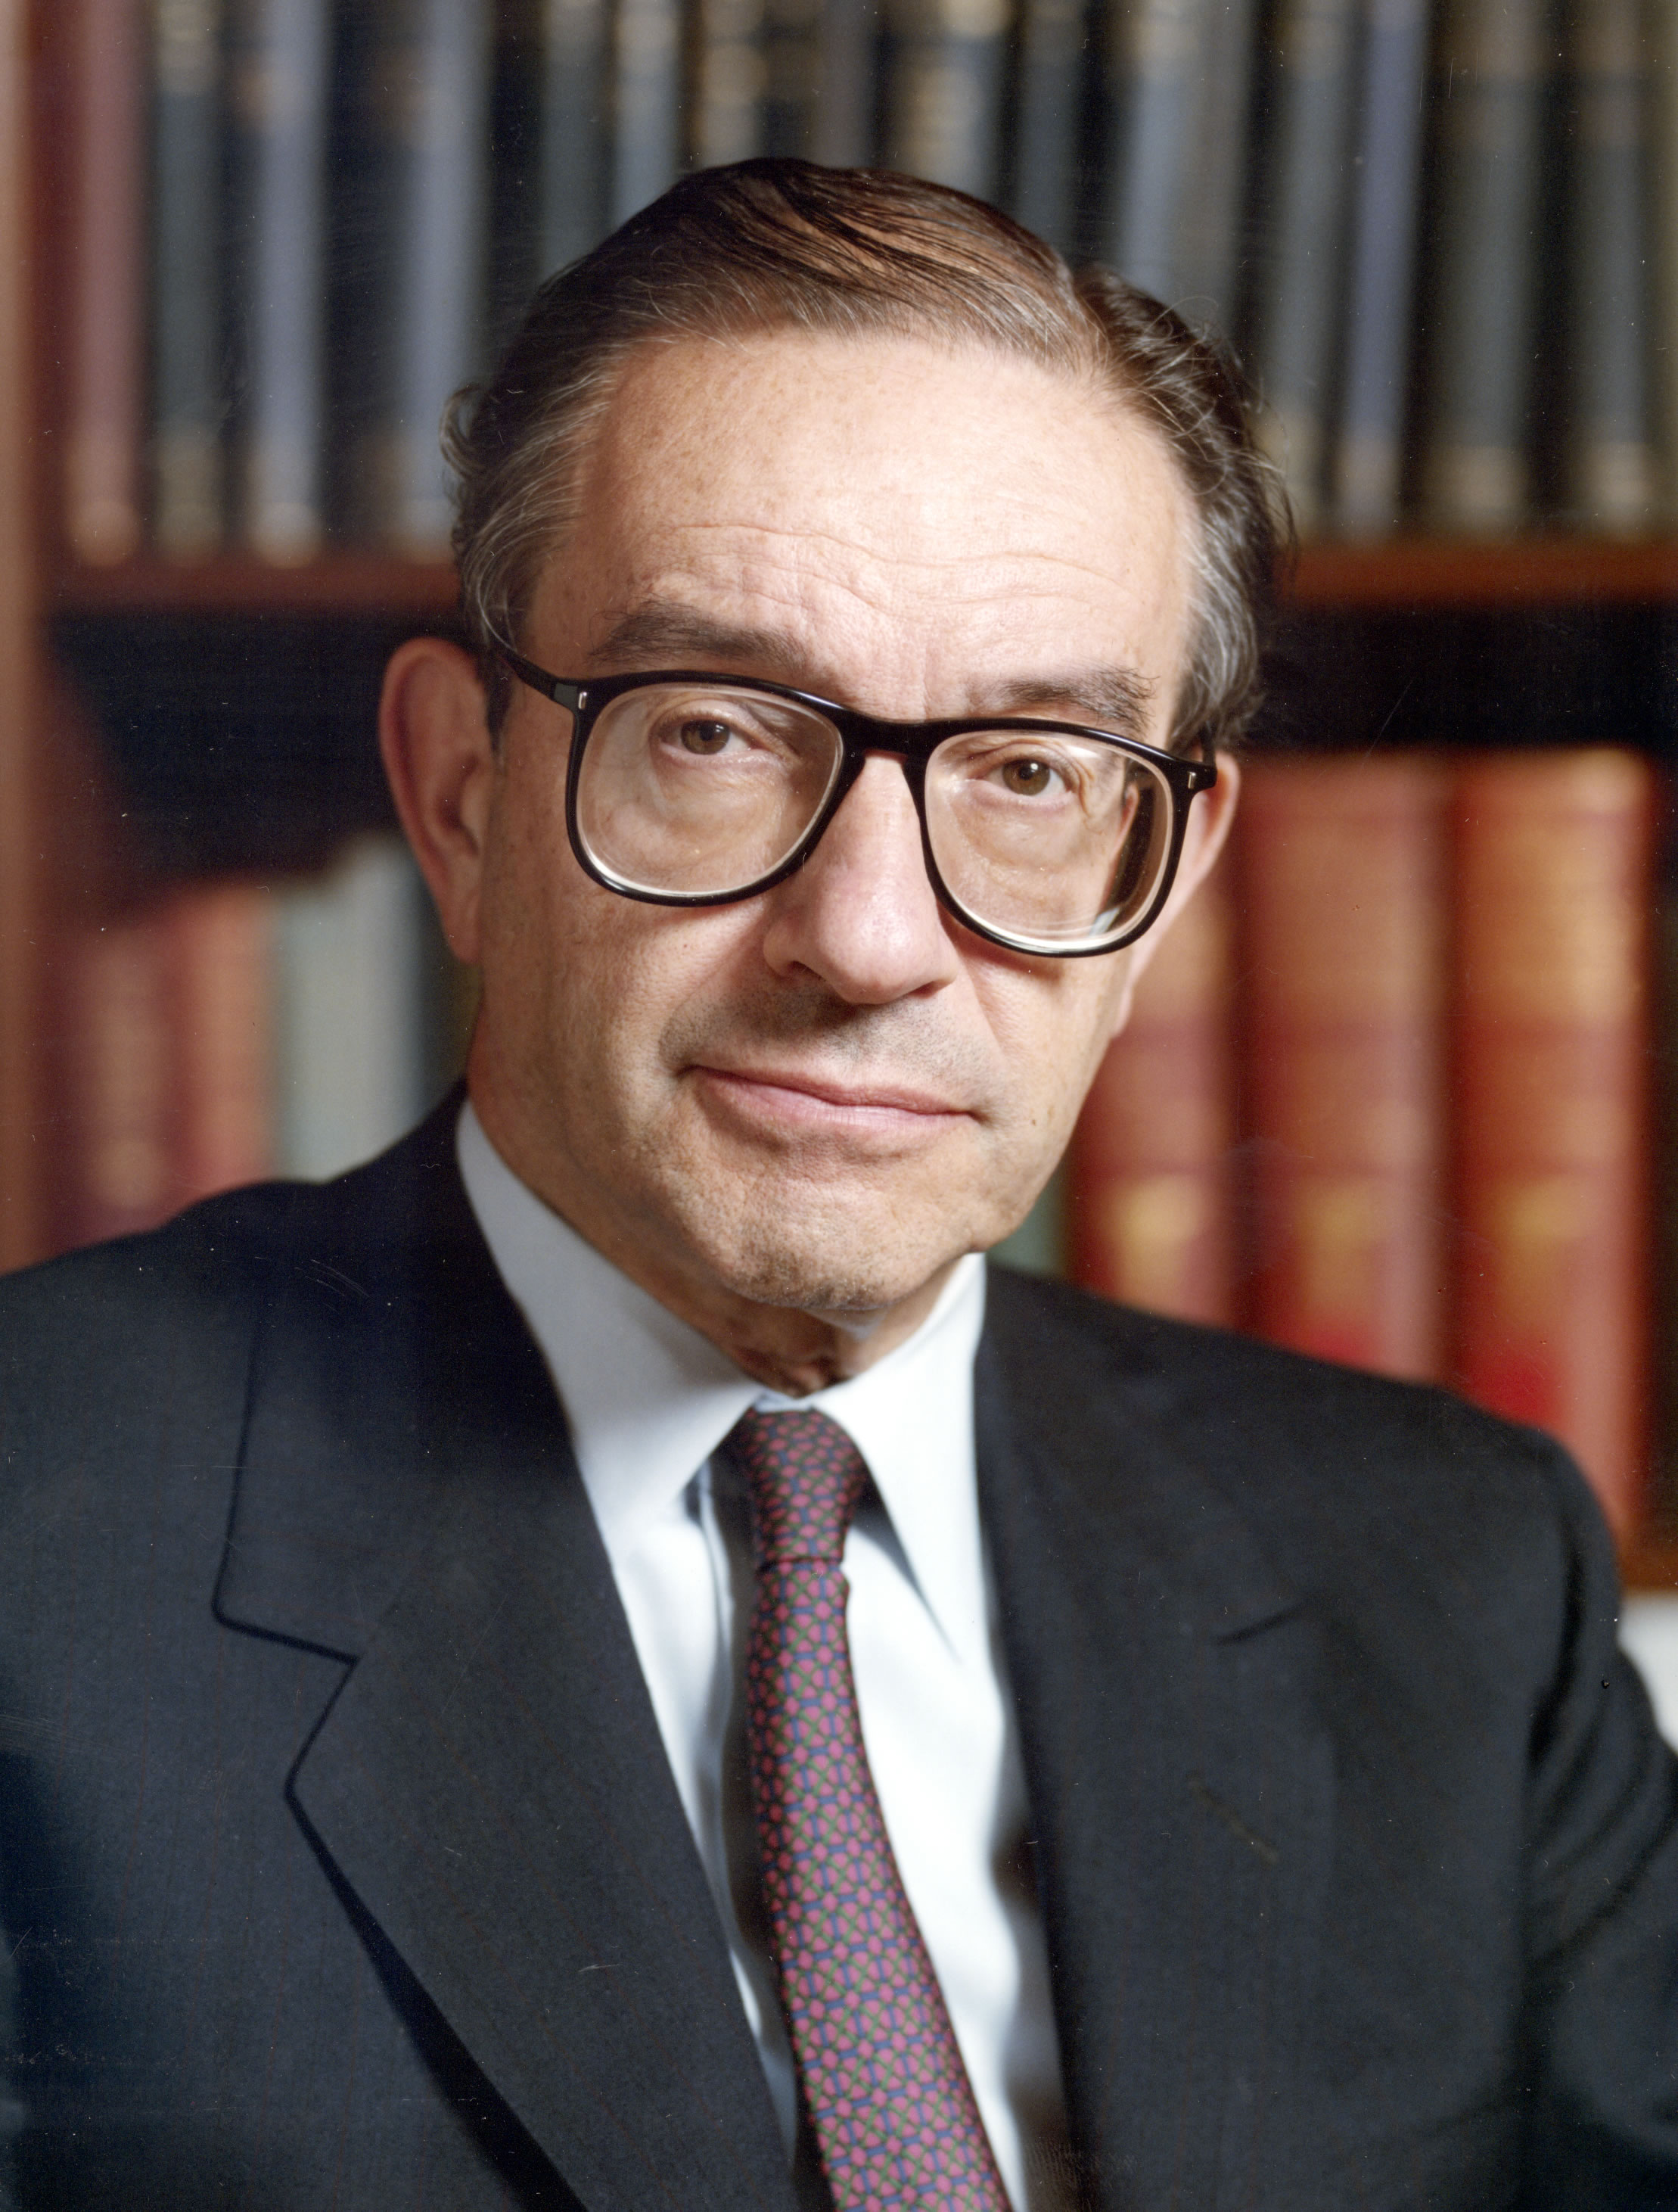
\includegraphics[width=5cm]{./alan_greenspan.jpg} \\
				\Large \textbf{- Alan Greenspan \cite{intro:bibliografia}}
			\end{center}
		\end{multicols}
		
	% * Insira também uma citação relativa ao tema.

	% * A consulta bibliográfica relativa ao tema e a citação são obrigatórias.


	% * Depois de toda a informação que consultou, em duas colunas, diga-nos
	% * o que descobriu com esta pesquisa, se acha vantajoso fazer e manter um orçamento atualizado.

	\begin{thebibliography}{99}
		\bibitem{intro:intro}
			\textbf{Associação de politécnicos do norte:}
				\url{https://bibliotecadigital.ipb.pt/bitstream/10198/24948/1/Catarina%20Marinho.pdf} \\
			\textbf{Congresso de Iniciação Científica:}
				\url{https://conic-semesp.org.br/anais/files/2015/1000021289.pdf}
		\bibitem{intro:desenvolvimento}
			\textbf{Jornal de Negocios:}
				\url{https://jornaldenegocios.pt/opiniao/deans-corner/joao-pinto/detalhe/mais-um-ano-letivo-a-arrancar-e-a-literacia-financeira} \\
			\textbf{Mapfre:}
				\url{https://mapfre.com/pt-br/actualidade/economia-pt-br/impacto-educacao-financeira-economia-pais/}
		\bibitem{intro:orcamento}
			\textbf{Forbes Portugal:}
				\url{https://forbespt.com/como-fazer-um-orcamento-pessoal/}
		\bibitem{intro:citacao}
			\textbf{O'REILLY}
				\url{https://www.oreilly.com/library/view/information-literacy-in/9781843345169/xhtml/B9781843345152500111.htm}
		\bibitem{intro:bibliografia}
			\textbf{Wikipedia:} \url{https://pt.wikipedia.org/wiki/Alan_Greenspan}
	\end{thebibliography}

\end{document}

% * Image bibliography
% * https://iconscout.com/illustration/finance-calculator-6771660
% * Quotes list
% * https://www.chime.com/blog/15-quotes-from-our-favorite-money-saving-experts/
% * https://www.brainyquote.com/quotes/john_w_rogers_jr_624550

